\asection{Introduction}
\label{Introduction}
Graphs are used in a variety of disciplines and they serve a multitude of purposes, such as representing the syntactical representations of the components in a sentence and their relationships to each other[10], describing the structures of chemical compounds in chemistry[11],representing the entries in a database and their relationships, pattern recognition and computer vision[2]. Thus because the digraph database structure is so widely used, it is important to find methods of finding the correlation between of data schemas in applications that make use of this comprehensive data structure[1]. This process is referred to as graph matching. Before we get to some of the graph matching algorithms, some concepts of graph theory must first be understood.\\\\
A Graph in Mathematics and Computer Science is a pair G = (V, E),  where V is the set of vertices and E is the set of edges, formed by pairs of vertices. Figure 1 demonstrates the structural attributes of a graph.

\begin{figure}[H]
  \begin{center}
      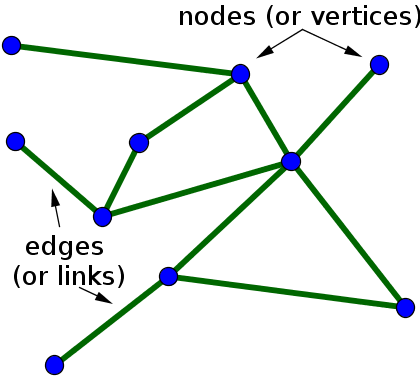
\includegraphics[width=0.65\textwidth]{graph.PNG}
  \end{center}    
  \caption{Representation of a graph}
\end{figure}

\begin{figure}[H]
  \begin{center}
      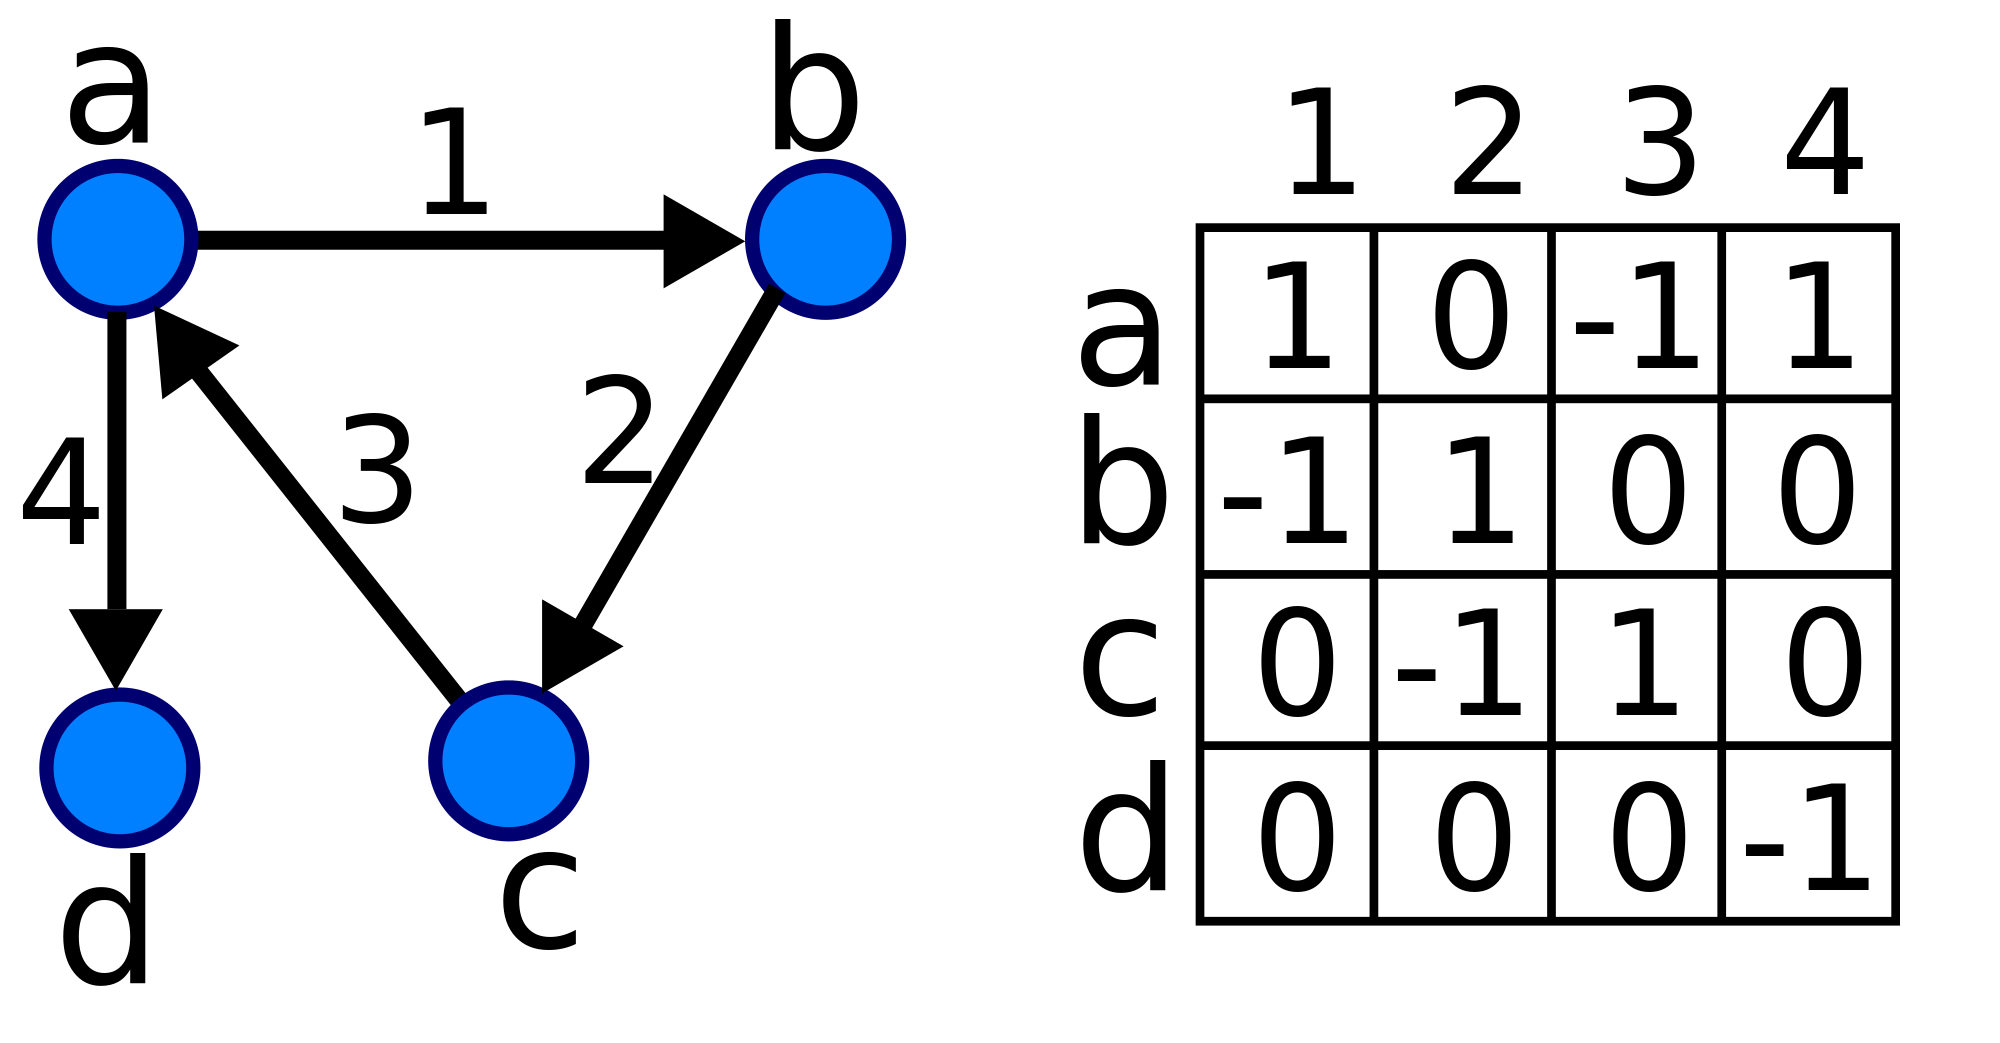
\includegraphics[width=0.65\textwidth]{digraph.PNG}
  \end{center}    
  \caption{Representation of a digraph}
\end{figure}

The graphs discussed in this paper are called directed graphs, refer to figure 2. Digraphs are graphs whose edges have a certain direction in which they are going, in figure 2 this characteristic is demonstrated by the edge 1, that goes from node a to node b, and also by edges 3 that goes from node c to node a. Note that in figure 1, the graph is referred to as a bigraph because the direction of its edges are in both ways as it is not specified.\\\\
Two graphs are said to be isomorphic if they are syntactically similar to each other iff there is a bijection between their respective nodes which make each edge of G1 correspond to exactly one edge of G2, and vice versa[12], i.e. the graphs are structurally the same to each other. This property is demonstrated in figure 3. The two graphs look very different, but when they are further inspected, it is evident that the two are a representation of the same data scheme or even the same graph that has been rearranged.

\begin{figure}[H]
  \begin{center}
      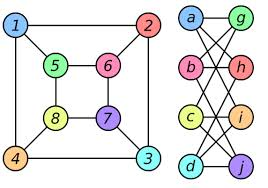
\includegraphics[width=0.65\textwidth]{isomorphism.PNG}
  \end{center}    
  \caption{Representation of the isomorphism property}
\end{figure}

Graphs are often represented as a matrix, more precisely a adjacency matrix. This is a nxn matrix A, with A(i,j) = 1 iff(i,j) ∈ E[12]. This means that wherever there is an edge in the graph, it is denoted by a 1 in the matrix, places in the matrix A where there is an absence of an edge E are denoted by 0.\\\\
Figure 4 depicts the association between a graph and its adjacency matrix.
\begin{figure}[H]
  \begin{center}
      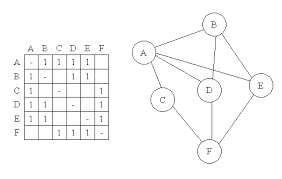
\includegraphics[width=0.65\textwidth]{matrix.PNG}
  \end{center}    
  \caption{Representation of a graph and its associated adjacency matrix}
\end{figure}

Lastly we introduce the concepts of sub graphs in Graph Theory. A graph G' = (V',E') is a sub graph of a graph G = (V, E) if V' ⊆ V and E' ⊆ E[12], i.e. the graph G' must appear inside graph G in order to be considered a sub graph of G.\\\\

A graph matching algorithm computes the association between two graphs, namely graph G' and G'' and measures the degree of this association.\\\\
 This paper analyses some of the more popular graph matching algorithms such as the Similarity Flooding[1] algorithms, VF[5], VF2[2], Ullman, Schmidt and Druffel algorithm[5] and the Nauty[5], specifically those that are tailored (designed) for digraphs, though most of these algorithm only perform syntactical (isomorphism) comparisons, we are going to investigate those algorithms that also perform semantic (content in the graphs) comparison or can be modified so that the existing algorithms can also be extended to perform semantic comparison.
